%SPDX-License-Identifer: CC-BY-SA-4.0
%License-Filename: LICENSE

\documentclass[hyperref, aspectratio=169]{beamer}

%\documentclass[handout]{beamer}
%\usepackage{pgfpages}
%\pgfpagesuselayout{2 on 1}[a4paper,border shrink=3mm]
%\pgfpagesuselayout{4 on 1}[a4paper,landscape,border shrink=3mm]

\usepackage[utf8]{inputenc}
\usepackage[ngerman]{babel}
\usepackage[T1]{fontenc}
\usepackage{lmodern}
\usepackage{uoscolor}
\usepackage{graphicx}
\usepackage{tikz}
\usetikzlibrary{positioning}
\usetikzlibrary{fit}
\usepackage{wrapfig}
\usepackage{floatflt,epsfig} 
%\usepackage{caption} 
\usepackage{eurosym}
\usepackage{subfigure}
\usepackage{units}
\usepackage{textcomp}

\usepackage{default}
\usepackage{pgfpages} %This is needed for notes presentation!
%\setbeameroption{show notes on second screen}

\usetheme{Berlin}


\setbeamercolor{section in toc}{fg=black,bg=white}
\setbeamercolor{alerted text}{fg=uos-red!80!gray}
\setbeamercolor*{palette primary}{   fg=uos-red,bg=white}
\setbeamercolor*{palette secondary}{ fg=uos-red,bg=white}
\setbeamercolor*{palette tertiary}{  bg=uos-red,fg=white}
\setbeamercolor*{palette quaternary}{fg=uos-red,bg=white}

\setbeamercolor*{sidebar}{fg=uos-red,bg=gray!15!white}

\setbeamercolor*{palette sidebar primary}{fg=uos-red!10!black}
\setbeamercolor*{palette sidebar secondary}{fg=white}
\setbeamercolor*{palette sidebar tertiary}{fg=uos-red!50!black}
\setbeamercolor*{palette sidebar quaternary}{fg=gray!10!white}

\setbeamercolor{titlelike}{parent=palette primary,fg=uos-red}
\setbeamercolor{frametitle}{bg=uos-gray!40!white}
\setbeamercolor{frametitle right}{bg=uos-grey}

\setbeamercolor*{separation line}{}
\setbeamercolor*{fine separation line}{}


\setbeamertemplate{itemize item}{\color{uos-red}$\blacksquare$}
\setbeamertemplate{itemize subitem}{\color{uos-red}$\blacktriangleright$}


\setbeamercolor{section number projected}{bg=uos-red,fg=white}


\setbeamertemplate{navigation symbols}{}
\title[Evaluierung eines Multiinstanz-Managers für 
prozessvirtualisierte Anwendungen am Beispiel von OpenSlides]{Evaluierung 
eines Multiinstanz-Managers für prozessvirtualisierte Anwendungen am Beispiel 
von OpenSlides} 
\subtitle{Oberseminar Informatik}
\author[Jochen Saalfeld]{}
\institute[University of Osnabrück]{
	
\includegraphics[width=0.38\textwidth]{unilogo}
}


\setbeamertemplate{footline}
{%
	\begin{beamercolorbox}[wd=1.0\textwidth,
			ht=2.6ex,
			dp=1ex,
			leftskip=.5em,
			rightskip=.5em]{author in head/foot}%
		\usebeamerfont{author in head/foot}%
		\insertshortauthor\hfill%\insertshortinstitute%
		%\insertframenumber{} von 
		%\inserttotalframenumber\hfill\insertshortauthor%
	\end{beamercolorbox}%
	%\hspace*{-4.0ex}\hspace*{0.3\textwidth}%
	\begin{beamercolorbox}[wd=1.0\textwidth,
			ht=2.6ex,
			dp=1ex,
			left,
			leftskip=.5em,
			rightskip=.5em]{title in head/foot}%
		\usebeamerfont{title in head/foot}%
		\insertshorttitle\hfill\insertframenumber{} / \inserttotalframenumber%
	\end{beamercolorbox}%
}

\begin{document}
%\date{\today}
\date{20.06.2018}
\frame{\titlepage}

\frame{\frametitle{Contents}\tableofcontents[ 
		currentsubsection, 
		hideothersubsections, 
		sectionstyle=show, 
		subsectionstyle=shaded 
	]
}
\section{Einführung}
\frame{\frametitle{Über mich}
	\begin{itemize}
		\item 28 Jahre alt
		\item 2011 Abitur an der BBS Brinkstraße in Osnabrück (Schwerpunkt IT)
		\item 2014 Abschluss als Fachinformatiker In Anwendungsentwicklung bei 
		Hellmann Worldwide Logistics
		\item 2014 - 2016 als Spezialist für Oracle Apex bei Hellmann
		\item 2016 beginn des Studiums in der Informatik an der Uni Osnabrück
		\item Seit 2016 als Softwareentwickler und -berater bei der freien 
		Software Firma Intevation in Osnabrück
		\begin{itemize}
			\item Gpg4win (BSI, g10code GmbH, Mailvelope, Enigmail \dots)
			\item OpenSlides
			\item \dots
		\end{itemize}
	\end{itemize}
}
\frame{\frametitle{Motivation}
	\begin{itemize}
		\item Hardware wird nicht vollständig benutzt (teuer)
			\begin{itemize}
				\item Eine Maschine pro Instanz vs. Mehrere Instanzen pro 
				Maschine
			\end{itemize}
		\item (Es existiert bereits ein Backend)
		\item Backend jedoch nicht mandantenfähig
		\item Technologie im existierenden Backend ist sehr komplex
		\item Skaliert nicht
	\end{itemize}
}
\frame{\frametitle{Suche nach Technolgien}
	\begin{itemize}
		\item Muss mandantenfähig sein
		\item Muss skalieren
		\begin{itemize}
			\item Mehrere Server
			\item Mehrere Instanzen
			\item Skalierbare und Anpassbare Instanzen
		\end{itemize}
		\item $\Rightarrow$ Orchestrierung
	\end{itemize}
}
\frame{\frametitle{Finden der Technologie}
	\begin{itemize}
		\item Prozessvirtualisierung und 
		\begin{itemize}
			\item \texttt{docker}, \texttt{rkt}, \texttt{rail-car}
		\end{itemize}
		\item Verwaltung der Prozesse
		\begin{itemize}
			\item \texttt{ansible}, \texttt{puppet}, \texttt{kubernetes}, 
			\texttt{docker swarm} (Teil von \texttt{docker})
		\end{itemize}
		\item Start mit \texttt{docker-compose} (Teil von \texttt{docker})
		\item Deployment in \texttt{docker swarm}
	\end{itemize}
}
\section{Architektur}
\frame{\frametitle{docker-compose}
	\begin{itemize}
		\item Schaffen lokalen \glqq{}Mini\grqq{}-Setups
		\item Anlegen von Volumen
		\item Anlegen von Netzwerken
		\item Verwaltung der Skalierung
	\end{itemize}
}
\frame{\frametitle{Instanz}
	\begin{itemize}
		\item \url{https://github.com/OpenSlides/openslides-docker}
		\item \textbf{Live-Demo}
	\end{itemize}
	\begin{center}
		\begin{tikzpicture}[node distance = 2.25cm,
							scale=0.7,
							every node/.style={scale=0.7}]
			\node [draw] (postgres) {postgres};
			\node [draw, left of=postgres] (redis) {redis}; 
			\node [draw, above left of=postgres] (core) {core};
			\node [draw, left of=redis] (worker1) {worker\_1};
			\node [draw, below=0.5cm of worker1] (worker2) {worker\_2};
			\node [below=0.1cm of worker2] (worker3) {$\vdots$};
			\node [draw, above left of=worker1] (postfix) {postfix};
			\node [draw, left of=worker1] (web1) {web\_1};
			\node [draw, below=0.5cm of web1] (web2) {web\_2};
			\node [below=0.1cm of web2] (web3) {$\vdots$};
			\node [draw, left of=web2] (nginx) {nginx};
			\node [draw, above of=nginx] (letsencrypt) {Let's Encrypt};
			\node [draw, below right=1cm and 1cm of nginx] (filesync) {filesync};
			\node [draw, right of=filesync] (pgslave) {pg-slave};
			\node[draw,
					inner sep=13mm,
					label=below:Network: back,
					fit=(filesync) (postgres) (core) (filesync) (web1)] {};
			\node[draw,
					inner sep=5mm,
					label=above:Network: front,
					fit=(letsencrypt) (nginx)] {};
			\path [->]
				(letsencrypt) edge [] (nginx)
				(nginx) edge [] (web1)
				(nginx) edge [] (web2)
				(web1) edge [] (worker1)
				(web1) edge [] (worker2)
				(web2) edge [] (worker1)
				(web2) edge [] (worker2)
				(postfix) edge [] (worker1)
				(worker1) edge [] (redis)
				(worker2) edge [] (redis)
				(redis) edge [] (postgres)
				(nginx) edge [] (filesync)
				(core) edge [] (postgres);
		\end{tikzpicture}
	\end{center}
}
\frame{\frametitle{Im Einsatz}
	\begin{center}
		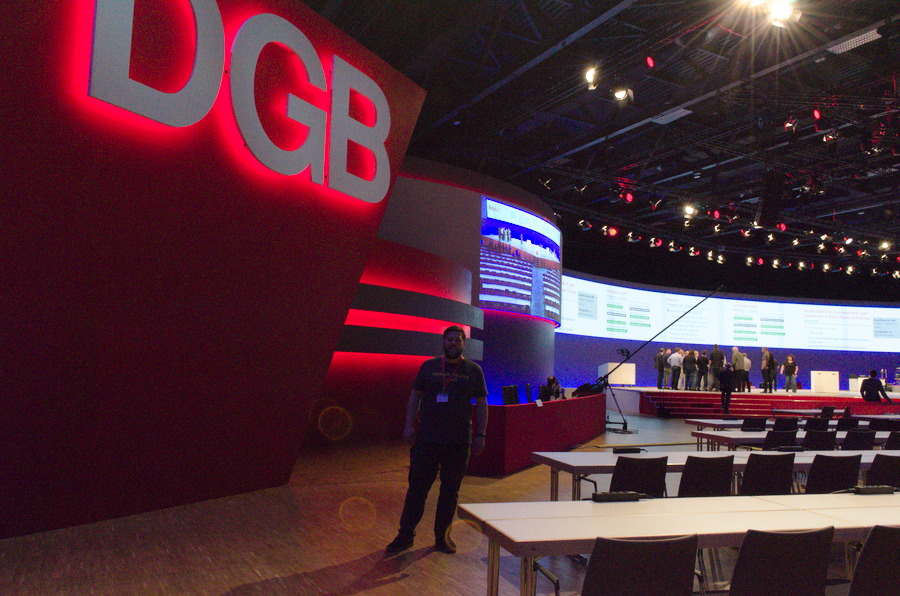
\includegraphics[scale=1]{img/DSC_1103.jpg}
	\end{center}
}
\frame{\frametitle{Im Einsatz}
	\begin{center}
		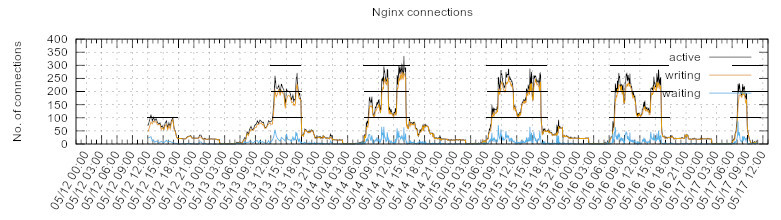
\includegraphics[scale=0.6]{img/total_nginx_scaled.jpg}
	\end{center}
}
\frame{\frametitle{Im Einsatz}
	\begin{center}
		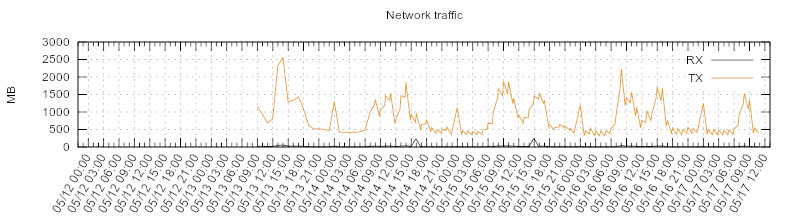
\includegraphics[scale=0.6]{img/total_network.jpg}
	\end{center}
}
\frame{\frametitle{Im Einsatz}
	\begin{center}
		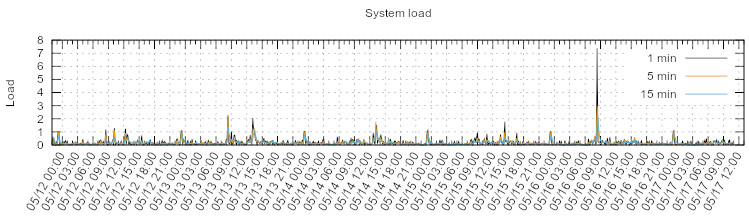
\includegraphics[scale=0.6]{img/total_load.jpg}
	\end{center}
}
\frame{\frametitle{Im Einsatz}
	\begin{center}
		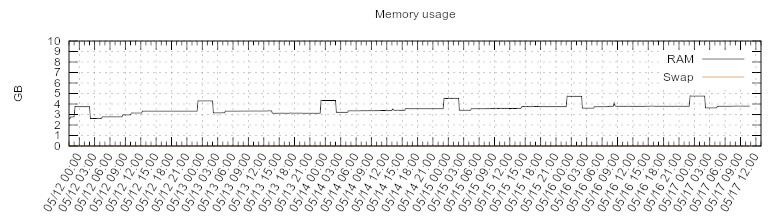
\includegraphics[scale=0.6]{img/total_memory.jpg}
	\end{center}
}
\frame{\frametitle{docker swarm}
	\begin{itemize}
		\item Gleiche Vorzüge wie \texttt{docker-compose}
		\item Einfach durch mehr Hardware erweiterbar
		\item Skaliert auch über Hardware
		\item Verteilt Last und Anforderungen automatisch
	\end{itemize}
}
\frame{\frametitle{Manager}
	\begin{itemize}
		\item \url{https://github.com/jsaalfeld/openslides-manager}
		\item \textbf{Live-Demo}
	\end{itemize}
	\begin{center}
		\begin{tikzpicture}[node distance = 2.5cm,
		scale=0.7,
		every node/.style={scale=0.7}]
		\node [draw] (nginx) {nginx};
		\node [draw, right of=nginx] (registry) {registry};
		\node [draw, above=0.1cm of registry] (frontend) {frontend};
		\node [draw, above=0.1cm of frontend] (backend) {backend};
		\node [draw, above=0.1cm of backend] (portainer) {portainer};
		\node [draw, below right=0.8cm and 1.5cm of frontend] (OS1) {OpenSlides 1};
		\node [draw, below=0.5cm of OS1] (OS2) {OpenSlides 2};
		\node [draw, below=0.5cm of OS2] (OS3) {OpenSlides 3};
		\node [below=0.1cm of OS3] (OS4) {\vdots};
		
		\node[draw,
			inner sep=7mm,
			label=below:Network: back,
			fit=(portainer) (registry)] {};
		\node[draw,
			inner sep=3mm,
			label=left:Network: front,
			fit=(nginx)] {};
		\node[draw,
			inner sep=4.mm,
			label=right:Network: OS1,
			fit=(OS1)] {};
		\node[draw,
			inner sep=4.1mm,
			label=right:Network: OS2,
			fit=(OS2)] {};
		\node[draw,
			inner sep=4.1mm,
			label=right:Network: OS2,
			fit=(OS3)] {};
		\path [->]
			(nginx) edge [] (portainer)
			(nginx) edge [] (backend)
			(nginx) edge [] (frontend)
			(nginx) edge [] (registry)
			(nginx) edge [bend right=35] (OS1)
			(nginx) edge [bend right=30] (OS2)
			(nginx) edge [bend right=25] (OS3);
		\end{tikzpicture}
	\end{center}
}
\section{Ausblick}
\frame{\frametitle{Ausblick}
	\begin{itemize}
		\item Wird im Rahmen der Arbeit stattfinden
		\item Automatisches Weiterleiten der Instanzen über \texttt{nginx} des 
		Managers
		\item Automatisches Zusenden von Backups
		\item wird nach der Arbeit noch Entwickelt
		\begin{itemize}
			\item Frontend zur Verwaltung der Instanzen mit Django
			\item Anbinden an ein Zahlungssystem
			\item Möglichkeit Backup-Instanzen in andere RZ zu deployen
		\end{itemize}
	\end{itemize}
}
\end{document}
